\chapter{Anhang}\label{ch:appendix}

\begin{listing}[htp]
  \begin{minted}[fontsize=\small]{yaml}
---
apiVersion: v1
kind: Pod
metadata:
  name: pod-exp
  namespace: namespace-exp
  labels:
    app: backend  
status:
  message: experiment
spec: 
  containers:
    - name: node-server
      image: nginx:stable-alpine
    \end{minted}
  \caption{pod.yaml auf Cluster ausgerollt}
  \label{lst:pod-yaml-file}
\end{listing}

\begin{listing}[htp]
  \begin{minted}[fontsize=\small]{yaml}
---
apiVersion: v1
kind Pod
metadata:
    name: pod-exp
  namespace: namespace-exp
  labels:
    app: backend
status:    
status:
  message: experiment
spec:
  containers:
    - name: node-server
      image: nginx:stable-alpine
    \end{minted}
  \caption{pod.yaml für Testfälle der Herausforderung 1}
  \label{lst:pod-yaml-file-1}
\end{listing}

\begin{listing}[htp]
  \begin{minted}[fontsize=\small]{yaml}
---
apiVersion: v1
kind: Pod
metadata:
  
  namespace: namespace-exp
  labels:
    app: backend
status:    
  message: experiment
  unknown: unknown  
spec:
  priority: high
    \end{minted}
  \caption{pod.yaml für Testfälle der Herausforderung 2}
  \label{lst:pod-yaml-file-2}
\end{listing}

\begin{listing}[htp]
  \begin{minted}[fontsize=\small]{yaml}
---
apiVersion: v1
kind: Pod
metadata:
  name: pod-exp
  namespace: namespace-exp
  labels:
    app: backend
status:    
  message: experiment 
spec:
  hostIPC: true
  hostNetwork: true
  hostPID: true
  volumes:
    - name: dockersocket
      hostPath:
        path: /var/run/docker.sock
  containers:
    - name: node-server
      image: nginx:stable-alpine
      env:
        - name: PASSWORD
          value: "super_secret_password"
        - name: ELASTIC
          value: "http://localhost:9200"
  \end{minted}
  \caption{pod.yaml für Testfälle der Herausforderung 3 - Version 1}
  \label{lst:pod-yaml-file-3-1}
\end{listing}

\begin{listing}[htp]
  \begin{minted}[fontsize=\small]{yaml}
---
apiVersion: v1
kind: Pod
metadata:
  name: pod-exp
  namespace: namespace-exp
  labels:
    app: backend
status:    
  message: experiment 
spec:
  containers:
    - name: node-server
      image: nginx:stable-alpine
      securityContext:
        allowPrivilegeEscalation: true
        capabilities:
          add:
            - CAP_SYS_ADMIN
            - CAP_SYS_MODULE
        privileged: true
  \end{minted}
  \caption{pod.yaml für Testfälle der Herausforderung 3 - Version 2}
  \label{lst:pod-yaml-file-3-2}
\end{listing}

\begin{listing}[htp]
  \begin{minted}[fontsize=\small]{yaml}
---
apiVersion: v1
kind: Pod
metadata:
  name: pod-exp
  namespace: 
  labels:
    app: backend
status:    
  message: experiment  
spec:
  containers:
    - name: node-server
      image: nginx:stable-alpine
  volumes:
    - name: secret-volume
      secret:
        secretName: secret-exp
    - name: secret-volume-2
      secret:
        secretName: unknown-secret
  \end{minted}
  \caption{pod.yaml für Testfälle der Herausforderung 4}
  \label{lst:pod-yaml-file-4}
\end{listing}

\begin{table}[htp]
  \centering
  \begin{tabularx}{\columnwidth}{lXXl}
    \toprule
    \begin{tabular}{@{}l@{}}\textbf{Name des} \\ \textbf{Programms} \end{tabular} & \begin{tabular}{@{}l@{}}\textbf{erfüllte}\\\textbf{Testfälle} \end{tabular} & \begin{tabular}{@{}l@{}}\textbf{nicht}\\\textbf{erfüllte}\\\textbf{Testfälle} \end{tabular} & \textbf{Anmerkungen}                                    \\
    \midrule
    \multirow{4}{*}{kubeconform}                                                  & 1.2                                                                         & 1.1, 1.3                                                                                    & Meldet ersten Syntaxfehler                              \\
                                                                                  & 2.1.1                                                                       & 2.1.2, 2.1.3, 2.2                                                                           & Meldet ersten Syntaxfehler                              \\
                                                                                  &                                                                             & 3                                                                                           &                                                         \\
                                                                                  &                                                                             & 4                                                                                           &                                                         \\
    \midrule
    \multirow{4}{*}{KubeLinter}                                                   &                                                                             & 1                                                                                           & Meldet, dass Validierung nicht erfolgreich war          \\
                                                                                  &                                                                             & 2                                                                                           & Meldet, dass Validierung nicht erfolgreich war          \\
                                                                                  & 3.1.1, 3.1.3{-}3.1.6, 3.1.8, 3.1.11                                         & 3.1.2, 3.1.7, 3.1.9, 3.1.10                                                                 &                                                         \\
                                                                                  &                                                                             & 4                                                                                           &                                                         \\
    \midrule
    \multirow{4}{*}{kube-score}                                                   & 1.2                                                                         & 1.1, 1.3                                                                                    & Meldet ersten Syntaxfehler                              \\
                                                                                  & 2.1.3                                                                       & 2.1.2, 2.1.3, 2.2                                                                           & Meldet ersten Syntaxfehler                              \\
                                                                                  & 3.1.1, 3.1.2, 3.1.11                                                        & 3.1.3{-}3.1.10                                                                              &                                                         \\
                                                                                  &                                                                             & 4                                                                                           &                                                         \\
    \midrule
    \multirow{4}{*}{kubectl-validate}                                             & 1.2                                                                         & 1.1, 1.3                                                                                    & Meldet ersten Syntaxfehler                              \\
                                                                                  & 2.1.2                                                                       & 2.1.1, 2.1.3, 2.2                                                                           & Meldet ersten Syntaxfehler                              \\
                                                                                  &                                                                             & 3                                                                                           &                                                         \\
                                                                                  &                                                                             & 4                                                                                           &                                                         \\
    \midrule
    \multirow{4}{*}{Lens}                                                         & 1.2                                                                         & 1.1, 1.3                                                                                    & Meldet ersten Syntaxfehler                              \\
                                                                                  &                                                                             & 2                                                                                           &                                                         \\
                                                                                  &                                                                             & 3                                                                                           &                                                         \\
                                                                                  &                                                                             & 4                                                                                           &                                                         \\
    \midrule
    \multirow{4}{*}{Monokle}                                                      & 1                                                                           &                                                                                             &                                                         \\
                                                                                  & 2.1.1, 2.1.3, 2.2                                                           & 2.1.2                                                                                       &                                                         \\
                                                                                  & 3.1.2{-}3.1.5, 3.1.7                                                        & 3.1.1, 3.1.6, 3.1.8{-}3.1.11                                                                &                                                         \\
                                                                                  & 4.1.2                                                                       & 4.1.1, 4.2                                                                                  & Softwarefehler bei der Validierung von \textit{Secrets} \\
    \midrule
    \multirow{4}{*}{\shortstack[l]{vscode-kubernetes-                                                                                                                                                                                                                                                                   \\tools}}                                      & 1                                                                           &                                                                                             &                                                         \\
                                                                                  & 2.1.1, 2.1.3, 2.2                                                           & 2.1.2                                                                                       &                                                         \\
                                                                                  & 3.1.1                                                                       & 3.1.2{-}3.1.11                                                                              &                                                         \\
                                                                                  &                                                                             & 4                                                                                           &                                                         \\
    \bottomrule
  \end{tabularx}
  \caption{Detaillierte Ergebnisse des Laborversuchs}
  \label{tbl:test-cases-experiment}
\end{table}


\begin{figure}[htp] % htp = hier (h), top (t), oder auf einer eigenen Seite (p).
  \centering
  \includesvg[width=0.8\textwidth]{images/language-service-interface.svg} % width immer angeben!
  \caption{Klassendiagramm des Interface ``LanguageService''}
  \label{fig:language-service-interface-defition}
\end{figure}

\vspace{0.5cm}

\begin{figure}[htp] % htp = hier (h), top (t), oder auf einer eigenen Seite (p).
  \centering
  \includesvg[width=0.35\textwidth]{images/class-diagram-json-document.svg} % width immer angeben!
  \caption{Klassendiagramm der Klasse ``JSONDocument''}
  \label{fig:class-diagram-json-document}
\end{figure}

\begin{figure}[htp] % htp = hier (h), top (t), oder auf einer eigenen Seite (p).
  \centering
  \includesvg[width=0.8\textwidth]{images/flowchart-get-node-from-offset.svg} % width immer angeben!
  \caption{Ablaufdiagramm der Methode ``getNodeFromOffset''}
  \floatfoot{Im Ablaufdiagramm steht ``CP'' für die Position des Cursors und ``K'' kann einen Knoten aus dem \ac{ast} eines
    \ac{yaml}-\textit{Documents} enthalten.}
  \label{fig:flowchart-get-node-from-offset}
\end{figure}


\begin{table}[htp]
  \centering
  \begin{tabular}{lllllllllll}
    \toprule
    \begin{tabular}{@{}l@{}}~\\~\\\\ \textbf{Kate-}\\ \textbf{gorie}\end{tabular} & \begin{tabular}{@{}l@{}} \emptycirc: nicht erfüllt \\ \fullcirc: erfüllt\\\\ \textbf{Kriterium} \end{tabular} & \rotatebox{90}{kubeconform} & \rotatebox{90}{KubeLinter} & \rotatebox{90}{kube-score} & \rotatebox{90}{kubectl-validate} & \rotatebox{90}{Lens} & \rotatebox{90}{Monokle} & \rotatebox{90}{vscode-kubernetes-tools} & \rotatebox{90}{ValidCube} & \rotatebox{90}{Eigene Implementierung} \\
    \midrule
    \multirow{7}{*}{1}                                                            & Interne Gründe                                                                                                & \fullcirc                   & \fullcirc                  & \fullcirc                  & \fullcirc                        & \emptycirc           & \fullcirc               & \fullcirc                               & \fullcirc                 & \fullcirc                              \\
                                                                                  & Folgen des Fehlers                                                                                            & \emptycirc                  & \emptycirc                 & \fullcirc                  & \emptycirc                       & \emptycirc           & \emptycirc              & \emptycirc                              & \emptycirc                & \emptycirc                             \\
                                                                                  & Beispiele zum Fehler                                                                                          & \emptycirc                  & \emptycirc                 & \emptycirc                 & \emptycirc                       & \emptycirc           & \emptycirc              & \emptycirc                              & \emptycirc                & \emptycirc                             \\
                                                                                  & Weitere Informationen                                                                                         & \fullcirc                   & \fullcirc                  & \emptycirc                 & \emptycirc                       & \emptycirc           & \fullcirc               & \fullcirc                               & \fullcirc                 & \emptycirc                             \\
                                                                                  & Kontext zum Fehler                                                                                            & \emptycirc                  & \fullcirc                  & \fullcirc                  & \fullcirc                        & \emptycirc           & \fullcirc               & \fullcirc                               & \fullcirc                 & \emptycirc                             \\
                                                                                  & Fehlercode                                                                                                    & \emptycirc                  & \emptycirc                 & \emptycirc                 & \emptycirc                       & \emptycirc           & \fullcirc               & \emptycirc                              & \fullcirc                 & \emptycirc                             \\
                                                                                  & Grundlegende Informationen                                                                                    & \emptycirc                  & \emptycirc                 & \fullcirc                  & \emptycirc                       & \emptycirc           & \fullcirc               & \emptycirc                              & \emptycirc                & \emptycirc                             \\
    \midrule
    \multirow{5}{*}{2}                                                            & Schnelle Fehlerbehebung                                                                                       & \emptycirc                  & \emptycirc                 & \emptycirc                 & \emptycirc                       & \emptycirc           & \emptycirc              & \emptycirc                              & \emptycirc                & \emptycirc                             \\
                                                                                  & Alternative Lösungen                                                                                          & \emptycirc                  & \emptycirc                 & \emptycirc                 & \emptycirc                       & \emptycirc           & \emptycirc              & \emptycirc                              & \emptycirc                & \emptycirc                             \\
                                                                                  & Vorschau zur Fehlerbehebung                                                                                   & \emptycirc                  & \emptycirc                 & \emptycirc                 & \emptycirc                       & \emptycirc           & \emptycirc              & \emptycirc                              & \emptycirc                & \emptycirc                             \\
                                                                                  & Beispiele zur Fehlerbehebung                                                                                  & \emptycirc                  & \emptycirc                 & \emptycirc                 & \emptycirc                       & \emptycirc           & \emptycirc              & \emptycirc                              & \emptycirc                & \emptycirc                             \\
                                                                                  & Anleitung zur Fehlerbehebung                                                                                  & \emptycirc                  & \fullcirc                  & \emptycirc                 & \emptycirc                       & \emptycirc           & \emptycirc              & \emptycirc                              & \fullcirc                 & \emptycirc                             \\
    \midrule
    \multirow{3}{*}{3}                                                            & Ausblenden von Fehlern                                                                                        & \emptycirc                  & \emptycirc                 & \emptycirc                 & \emptycirc                       & \emptycirc           & \emptycirc              & \emptycirc                              & \emptycirc                & \emptycirc                             \\
                                                                                  & Punktesystem                                                                                                  & \emptycirc                  & \emptycirc                 & \emptycirc                 & \emptycirc                       & \emptycirc           & \emptycirc              & \emptycirc                              & \emptycirc                & \emptycirc                             \\
                                                                                  & Nutzerwissen zur Einordnung                                                                                   & \emptycirc                  & \emptycirc                 & \emptycirc                 & \emptycirc                       & \emptycirc           & \emptycirc              & \emptycirc                              & \emptycirc                & \emptycirc                             \\
    \midrule
    \multirow{4}{*}{4}                                                            & Anpassung der Regeln                                                                                          & \fullcirc                   & \fullcirc                  & \emptycirc                 & \emptycirc                       & \emptycirc           & \emptycirc              & \emptycirc                              & \emptycirc                & \emptycirc                             \\
                                                                                  & Verarbeitung von Fehlern                                                                                      & \emptycirc                  & \emptycirc                 & \emptycirc                 & \emptycirc                       & \fullcirc            & \fullcirc               & \emptycirc                              & \emptycirc                & \emptycirc                             \\
                                                                                  & temporäres Ausblenden                                                                                         & \emptycirc                  & \emptycirc                 & \fullcirc                  & \emptycirc                       & \emptycirc           & \emptycirc              & \emptycirc                              & \emptycirc                & \emptycirc                             \\
                                                                                  & Filter zum Ausblenden                                                                                         & \fullcirc                   & \fullcirc                  & \fullcirc                  & \emptycirc                       & \emptycirc           & \emptycirc              & \emptycirc                              & \emptycirc                & \emptycirc                             \\
    \midrule
    \multirow{3}{*}{5}                                                            & Priorisierung von Fehlern                                                                                     & \emptycirc                  & \emptycirc                 & \emptycirc                 & \emptycirc                       & \emptycirc           & \fullcirc               & \emptycirc                              & \emptycirc                & \emptycirc                             \\
                                                                                  & \ac{ide}-Integration                                                                                          & \emptycirc                  & \emptycirc                 & \emptycirc                 & \emptycirc                       & \emptycirc           & \fullcirc               & \fullcirc                               & \emptycirc                & \fullcirc                              \\
                                                                                  & Rückmeldung bei Fehlerbehebung                                                                                & \emptycirc                  & \emptycirc                 & \emptycirc                 & \emptycirc                       & \emptycirc           & \emptycirc              & \emptycirc                              & \emptycirc                & \emptycirc                             \\
    \midrule
    \multirow{4}{*}{6}                                                            & Markieren von Fehlern und Warnsymbole                                                                         & \emptycirc                  & \emptycirc                 & \emptycirc                 & \emptycirc                       & \emptycirc           & \fullcirc               & \fullcirc                               & \emptycirc                & \fullcirc                              \\
                                                                                  & Übersicht von Fehlermeldungen                                                                                 & \emptycirc                  & \emptycirc                 & \emptycirc                 & \emptycirc                       & \emptycirc           & \fullcirc               & \fullcirc                               & \emptycirc                & \fullcirc                              \\
                                                                                  & Historie der bereits behobenen Fehler                                                                         & \emptycirc                  & \emptycirc                 & \emptycirc                 & \emptycirc                       & \emptycirc           & \emptycirc              & \emptycirc                              & \emptycirc                & \emptycirc                             \\
                                                                                  & Suche von Fehlern                                                                                             & \emptycirc                  & \emptycirc                 & \emptycirc                 & \emptycirc                       & \emptycirc           & \fullcirc               & \fullcirc                               & \emptycirc                & \fullcirc                              \\

    \bottomrule
  \end{tabular}
  \caption{Detaillierte Ergebnisse des Vergleichs}
  \label{tbl:comparison-of-tools}
\end{table}


\begin{figure}[htp] % htp = hier (h), top (t), oder auf einer eigenen Seite (p).
  \centering
  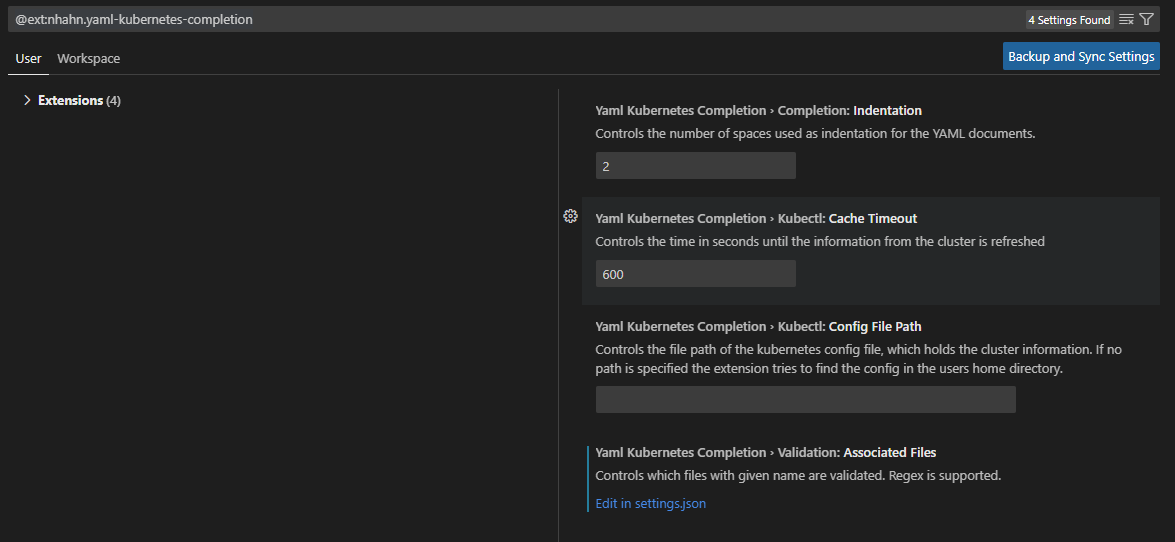
\includegraphics[width=1.0\textwidth]{images/screenshot-settings.png} % width immer angeben!
  \caption{Bildschirmaufnahme der Einstellungen der Anwendung}
  \label{fig:screenshot-settings}
\end{figure}

\begin{figure}[htp] % htp = hier (h), top (t), oder auf einer eigenen Seite (p).
  \centering
  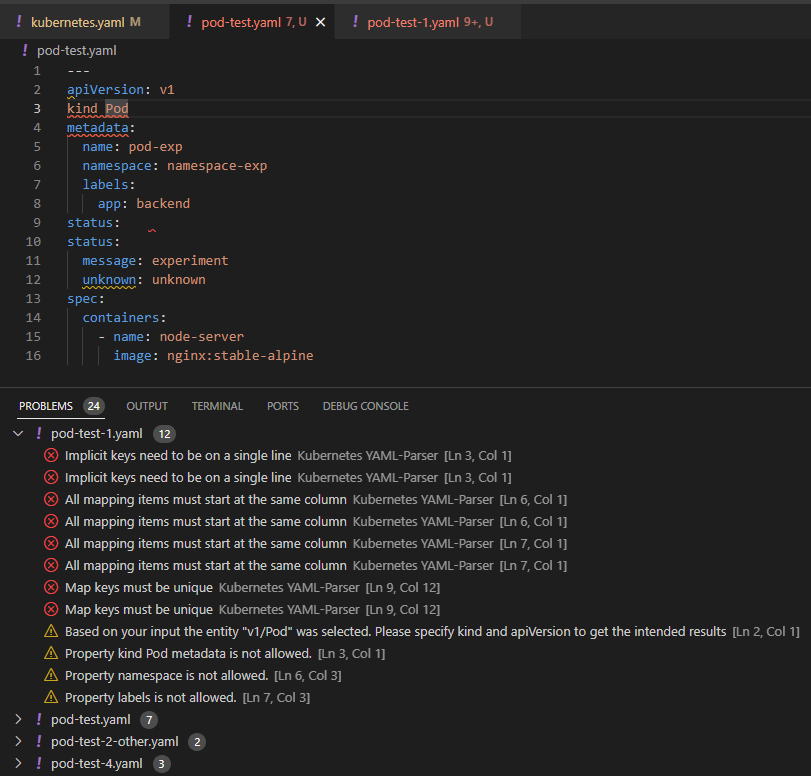
\includegraphics[width=0.8\textwidth]{images/screenshot-validation.png} % width immer angeben!
  \caption{Bildschirmaufnahme einer Datei mit Fehlern einer Validierung}
  \label{fig:screenshot-validation}
\end{figure}

\begin{figure}[H] % htp = hier (h), top (t), oder auf einer eigenen Seite (p).
  \centering
  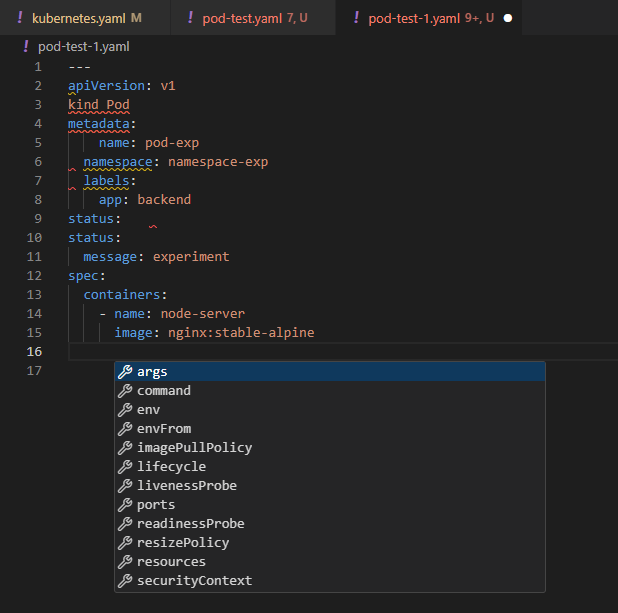
\includegraphics[width=0.8\textwidth]{images/screenshot-completion.png} % width immer angeben!
  \caption{Bildschirmaufnahme einer Datei mit Vorschlägen zur Autovervollständigung}
  \label{fig:screenshot-completion}
\end{figure}




